\documentclass{article}
\usepackage[T1]{fontenc}
\usepackage{lmodern}
\usepackage{graphicx}
\usepackage{amsmath,amssymb}
\usepackage[a4paper,margin=2cm]{geometry}
\usepackage[absolute,overlay]{textpos}
\setlength{\TPHorizModule}{1mm}
\setlength{\TPVertModule}{1mm}
\usepackage[indonesian]{babel}
\usepackage{hyperref}
\setlength{\emergencystretch}{2em}
% unit: Halaman 57

\begin{document}

% === Halaman 57 (llm) ===

\vspace{237.01mm}

\section*{Kriptografi pada Perang Dunia II}

\begin{itemize}
    \item Perang Dunia ke II, Pemerintah Nazi Jerman membuat mesin enkripsi yang dinamakan \textit{Enigma}.
    \item \textit{Enigma cipher} berhasil dipecahkan oleh pihak Sekutu.
    \item Keberhasilan memecahkan \textit{Enigma} sering dikatakan sebagai faktor yang memperpendek perang dunia ke-2
\end{itemize}

\vspace{20mm}

\begin{center}
    Enigma
\end{center}

% deskripsi: Foto mesin Enigma dengan berbagai label keterangan bagian-bagian mesin seperti spare light bulbs, viewing windows, rotor cylinder, position of rotors, plugboard, keyboard, dan alphabetical lightboard.
% bbox normalisasi: [0.5370, 0.0740, 0.9660, 0.8720]
\begin{textblock*}{90.09mm}(112.77mm,21.98mm)
\noindent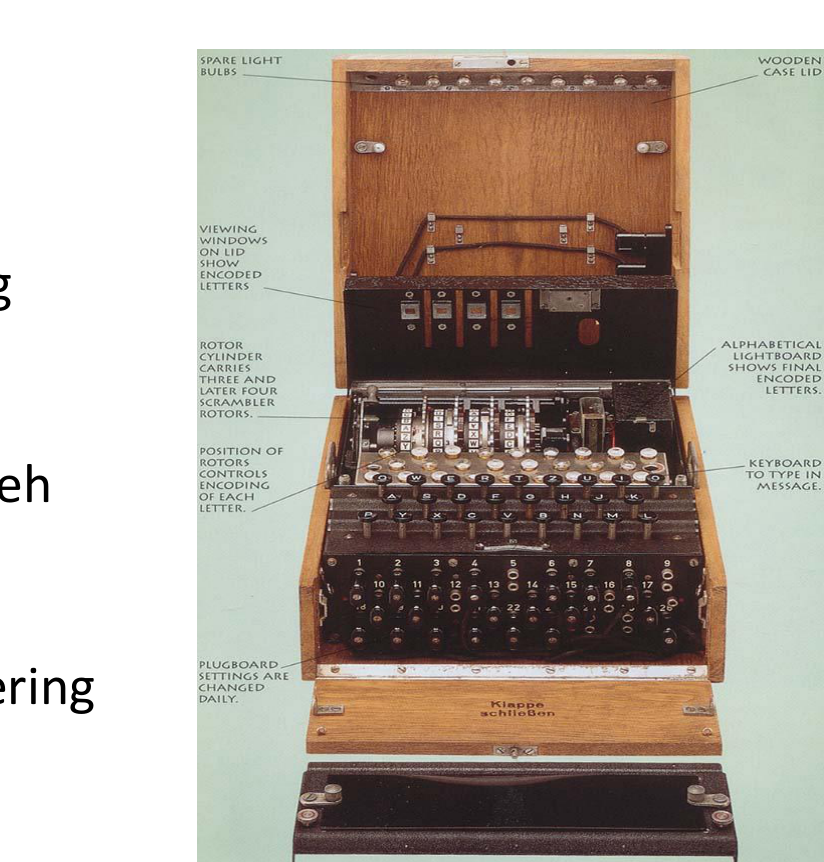
\includegraphics[width=90.09mm,height=237.01mm]{../../images/llm/page_057_img_01.png}%
\end{textblock*}

\end{document}
